\section{Evaluation}
\label{sec:eval}
To evaluate the effectiveness of \sysname{}, we assess its performance across a range of real-world and synthetic network configurations. Our evaluation is structured around four key research questions:
%, which allow us to examine \sysname{}'s capabilities under both targeted and open-ended conditions and to compare its behavior against state-of-the-art detection methods.

%The evaluation will address the following questions in order:
\begin{enumerate}
    \item Can \sysname{} accurately detect known misconfigurations in controlled and real-world settings?
    \item Can \sysname{} identify novel, previously unknown issues in large-scale networks?
    \item What types of contextual information do different Large Language Models (LLMs) request when diagnosing issues, and how does this affect their performance?
    \item How does \sysname{}'s detection capability compare to existing state-of-the-art verification tools?
\end{enumerate}

%We now describe the datasets and experimental setup used to address these questions, followed by detailed findings in the subsequent sections.

\subsection{Evaluation Setup}

\mypara{Datasets:}
Our evaluation uses three distinct sets of network configurations obtained from a nationwide Research \& Education Network (Internet2), a medium-scale campus network (Campus A), and a large-scale campus network (Campus B). We sample representative routers from each environment for evaluation. Table~\ref{tab:dataset_summary} provides an overview of these datasets.



\begin{table}[t]
\centering
\resizebox{\columnwidth}{!}{
\begin{tabular}{|l|l|c|l|r|r|}
\hline
\multirow{2}{*}{\textbf{Dataset}} & \multirow{2}{*}{\textbf{Vendor(s)}} & \textbf{No. Devices} & \multirow{2}{*}{\textbf{Device Roles}} & \multicolumn{2}{c|}{\textbf{Avg. Config Length}} \\
\cline{5-6}
& & \textbf{Sampled} & & \textbf{Lines} & \textbf{Tokens} \\ \hline
Internet2 & Juniper & 17 & TBA & ~18,944 &  \\
Campus A & Aruba & 8 & TBA & ~5,563 & \\
Campus B & Cisco, Juniper & 5 & Distribution \& Aggregation Routers & ~6,261 & \\ \hline
\end{tabular}
}
\caption{Overview of Network Configurations Used in Evaluation.}
\label{tab:dataset_summary}
\end{table}

\mypara{Context Extraction Hardware:}
The machine we use for context extraction has a single AMD EPYC 7302P (3GHz, 16-Core/32-Thread, 128MB L3 cache) processor and 64GB of memory. We do not use GPU acceleration, because \sysname{}'s context extraction and orchestration logic is CPU-parallelizable and does not significantly benefit from the GPU.

\mypara{Querying LLMs:}
We evaluate \sysname{} using GPT-4o~\cite{achiam2023gpt}
%OpenAI's latest model optimized for complex reasoning and long-context tasks 
(context window: 128,000 tokens; max output: 4,096 tokens; training cutoff: October 2023)
and DeepSeek-V3 (DS)~\cite{deepseekai2024deepseekv3technicalreport}
%DeepSeek-AI's open-source transformer suited for structured code and configuration analysis
(context window: 128,000 tokens; max output: 8,000 tokens; training cutoff: July 2024). For all experiments, we use the official chat completions APIs. This API is inherently stateless, which is critical for reproducibility, as each call is an independent event. To enable our iterative diagnostic process, our framework simulates a stateful conversation by constructing a complete, ordered history for each new query. Specifically, every API call includes the full sequence of prior prompts, the model's requests for context, the context provided by \sysname{}, and the model's intermediate reasoning steps. This method provides the best of both worlds: the controlled, reproducible environment of a stateless API, and the sophisticated, multi-step reasoning of a stateful dialogue, with our framework maintaining full control over the conversational history at every step.

\subsection{Can \sysname{} Detect Known Misconfigurations?}

We first evaluate \sysname{}'s effectiveness in detecting misconfigurations with a known ground truth. This is a crucial baseline for establishing accuracy. We conduct this analysis in two distinct settings: first, using synthetically generated but realistic errors injected into production configurations from Internet2, and second, using real, known misconfigurations from the Campus A network.

\mypara{Detecting Synthetic Misconfigurations in Internet2:}
To create a controlled environment for measuring detection performance, we obtained snapshot configurations from Internet2 (Juniper devices) and introduced 32 updates, comprising 16 correct updates (the original lines of config) and 16 erroneous modifications. These errors, inspired by misconfigurations identified in prior work~\cite{some_prior_work}, are categorized into three types:

\begin{itemize}
    \item \textit{Syntax errors} occur when the configuration does not adhere to the expected format or structure---\eg, a missing bracket or misused keyword in a BGP routing policy.
    \item \textit{Range violations} involve parameter values that fall outside the acceptable range---\eg, an MTU value that exceeds the maximum allowed for a specific interface type.
    \item \textit{Dependency/conflict (D/C) issues} arise when different configuration lines are incompatible or contradict each other. This broad category covers both dependency errors (\eg, a reference to a non-existent group) and consistency/conflict errors (\eg, a firewall rule that blocks traffic another policy explicitly permits).
\end{itemize}

For syntax and range errors, we created four distinct misconfigurations each. For D/C misconfigurations, we introduced eight distinct errors, as vanilla LLMs often excel at detecting localized syntax and range issues, while \sysname{}’s context mining is particularly effective for uncovering nuanced D/C issues that require broader understanding. The additional D/C errors allow us to thoroughly assess this core capability. Table~\ref{tab:syn_configs} provides details on these errors. Note that some errors involve Juniper's `apply-groups` feature, a unique mechanism for configuration inheritance that can challenge tools not specifically designed to reason about it.

For this case study, the \sysname{} implementation is powered by \textbf{GPT-4o}. For each update, we run \sysname{} by treating the modified line as the line under review and conducting the iterative prompting process. 
%Based on our finding that asking the model to search for `GENERAL` misconfigurations led to successful detection, we used this simpler, more general prompt for the analysis, rather than prompting for specific error types individually. 
To provide qualitative insight into the detection process, Table~\ref{tab:syn_responses} in Appendix~\ref{subsec:example_llm_reasoning} shows representative examples of the reasoning provided by the LLM when identifying several of the misconfigurations.



The results of this case study demonstrate the effectiveness of our iterative, context-aware approach. \sysname{} successfully identified all 16 synthetic misconfigurations while correctly validating all 16 correct updates, achieving 100\% accuracy with zero false positives or false negatives.
The analysis of the requested context in Table~\ref{tab:syn_configs} reveals a key insight into this success. For simple, self-contained syntax errors like a missing brace, the LLM correctly determined that no additional context was needed to identify the issue. However, for more complex range and D/C errors, the model consistently requested the precise contextual information required for a correct diagnosis. For instance, to validate a prefix limit (`Range' error) or a policy (`D/C' error), it asked for definitions and similar lines (R(P) and S(P)). This confirms that the two-step process—where the model first identifies and requests necessary evidence before making a final judgment—is critical for achieving high accuracy on nuanced configuration errors that are impossible to detect from a single line in isolation.

\begin{table}[tb]
\centering
\resizebox{\columnwidth}{!}{
\begin{tabular}{|l|l|l|l|}
\hline
\textbf{Type} & \textbf{Description} & \textbf{Misconfig Example} & \textbf{Requested Context}\\ \hline

\multirow{4}{*}{\textbf{Syntax}} 
& Missing closing brace &...interfaces: \{\textcolor{red}{"<ge-*"}: & None\\ \cline{2-4}
& Invalid keyword for value & ...mtu: \textcolor{red}{"True"}    & \( N(P) \), \( R(P) \)\\ \cline{2-4}
& Incorrect hierarchical placement & ...host-name: \textcolor{red}{"\{rtsw.alba-re1\}"}  & \( N(P) \)\\ \cline{2-4}
& Invalid IP address format & ...neighbor: \textcolor{red}{192.168.253.1.1}" & \( N(P) \), \( R(P) \)\\ \hline

\multirow{4}{*}{\textbf{Range}}  
& MTU exceeds interface max & ...mtu: \textcolor{red}{"10000"}  & \( N(P) \), \( R(P) \)\\ \cline{2-4}
& VLAN ID outside standard 1-4094 range & ...vlan-id: \textcolor{red}{"5000"}  & \( N(P) \), \( R(P) \), \( R(N(P)) \) \\ \cline{2-4}
& AS number outside valid range & ...autonomous-system: \textcolor{red}{70000} & \( N(P) \), \( R(P) \) \\ \cline{2-4}
& Prefix limit exceeds typical values & ...maximum: \textcolor{red}{"200000"} & \( N(P) \), \( R(P) \)  \\ \hline

\multirow{8}{*}{\textbf{D/C}}  
& Reference to a non-existent group & ... apply-groups: \textcolor{red}{"L2-LSP-ATTRIBUTES”} & \( N(P) \), \( R(P) \), \( R(N(P)) \) \\ \cline{2-4}
& Contradictory actions in a policy & ...community \textcolor{red}{add I2CLOUD-EXTENDED-TARGET}  & \( N(P) \), \( R(P) \), \( R(N(P)) \) \\ \cline{2-4}
& Reference to a non-existent filter & ...input-list: \textcolor{red}{"uplink"} & \( N(P) \), \( R(P) \)  \\ \cline{2-4}
& Reference to a non-existent policy & ...export: \textcolor{red}{"OESS-400-300-LOOP} & \( R(P) \)  \\ \cline{2-4}
& Applying an IPv6 filter to MPLS family & ...family mpls: filter:input-list:\textcolor{red}{"v6filter"} & \( R(P), S(P) \)  \\ \cline{2-4}
& Sampling disabled for one protocol family & ...family inet6: \textcolor{red}{SAMPLING MISSING/DISABLED}& \( R(P), N(P) \)  \\ \cline{2-4}
& Mismatch between VRF target and RD & ...vrf-target target:11537:\textcolor{red}{"313001"}& \( S(P) \)  \\ \cline{2-4}
& Unusually small MTU for ISO family & ...family iso: mtu: \textcolor{red}{"1497"}& \( R(P), S(P) \)  \\ \hline
\end{tabular}}
\caption{Erroneous Configuration Updates Introduced and LLM Requested Context for \sysname{}. The descriptions have been clarified to explain the nature of each error.}
\label{tab:syn_configs}
\end{table}



% \begin{table}[ht]
% \centering
% \resizebox{\columnwidth}{!}{
% \begin{tabular}{|l|l|l|p{8cm}|} % Define a fixed width for the Reason column
% \hline
% \textbf{Type} & \textbf{Misconfig} & \textbf{errParameter} & \textbf{Reason}\\ \hline

% \multirow{3}{*}{\textbf{Syntax}} & \multirow{3}{*}{Missing brace} & \multirow{3}{*}{["<ge-*>"]} & "MTU value for 'family inet' is set to 9174 which is less than the interface MTU value of 9192. The MTU for 'family inet' should not be less than the interface MTU."\\\hline

% \multirow{4}{*}{\textbf{Range}} & \multirow{4}{*}{Invalid VLAN ID} & \multirow{3}{*}{["maximum"]} & "The 'maximum' value of 200000 in the configuration line under review significantly exceeds the 'maximum' values of 1000 found in similar configuration lines, indicating a potential range misconfiguration."\\\hline

% \multirow{20}{*}{\textbf{D/C}} & \multirow{5}{*}{Policy Conflict} & \multirow{5}{*}{["remove-comms-rt"]} & "There is a conflict in the configuration under term 'remove-comms-rt' where the action 'community add I2CLOUD-EXTENDED-TARGET' is followed by 'community delete I2CLOUD-EXTENDED-TARGET' which are contradictory actions."\\\cline{2-4}

%  & \multirow{5}{*}{Disabled Sampling} & \multirow{5}{*}{["inet6"]} & "The family mpls is incorrectly using the IPv6 filter inet6-sample v6filter, which is intended for family inet6 in similar configuration lines. MPLS traffic should have its own specific filter, as the filtering requirements for MPLS are different from those for IPv6."\\\cline{2-4}
%  & \multirow{5}{*}{VRF Target Conflict} & \multirow{5}{*}{["target"]} & "The route-distinguisher (RD) in neighoring configurations is set to 11537:381841, while the vrf-target is set to target:11537:313001. These values should typically align, or at least follow certain conventions for mapping VRFs to the correct target instances in MPLS/BGP L2VPN."\\\cline{2-4}
%  & \multirow{5}{*}{Incorrect Filter Usage} & \multirow{5}{*}{["input-list"]} & "The family mpls is incorrectly using the IPv6 filter inet6-sample v6filter, which is intended for family inet6 in similar configuration lines. MPLS traffic should have its own specific filter, as the filtering requirements for MPLS are different from those for IPv6."\\\hline
% \end{tabular}}
% \caption{Example LLM Reasoning for \sysname{}.}
% \label{tab:syn_responses}
% \end{table}

\mypara{Detecting Known Misconfigurations in Campus A:}
To complement the synthetic analysis, we test \sysname{}'s ability to find known, real-world misconfigurations in the Campus A network. The network operators for this campus were specifically interested in detecting incorrect `VLAN assignments'—a type of misconfiguration that often requires a network-wide view, as deviations from uniform configurations across devices can indicate potential issues.
 This scenario demonstrates \sysname{}'s flexibility and we used both the \textbf{GPT-4o} and \textbf{DeepSeek-V3} backends.
 
 % To detect this specific issue, we augmented its default context library with a custom `Inter-Router Consistency Context', which mines the prevalence of a parameter-value pair across all other devices in the network.
 
 % For this analysis, we used both the \textbf{GPT-4o} and \textbf{DeepSeek-V3} backends.

In this targeted analysis, \sysname{} demonstrated perfect accuracy, correctly identifying all 6 known cases of incorrect VLAN assignments (100\% true positive rate). Both LLM backends yielded identical results. Among the six detected cases, two were previously unnoticed yet genuine misconfigurations that had been causing misrouting and network access issues, representing high-severity problems for network operations. The remaining four cases were intentional, benign misconfigurations applied to test and experimental devices.



\subsection{Can \sysname{} Accurately Identify New Issues?}

Beyond detecting known error types, a key goal for \sysname{} is to discover latent or novel misconfigurations in large, complex networks. To evaluate this capability, we performed a comprehensive verification of configuration snapshots from Campus A (Aruba devices) and Campus B (Cisco and Juniper devices). 
%Unlike the previous tests, no update information or error hints were provided. Instead, \sysname{} was instructed to exhaustively analyze full configurations to surface any deviations from general policy correctness and best practices.
In particular, each line of configuration from a subset of devices was fed to \sysname{} to determine if it contained an error.
For each misconfiguration detected by \sysname{}, we verified the correctness of the inference with domain experts from the respective campus networks. 
This open-ended approach allows us to not only assess \sysname{}'s scalability and discovery potential but also to evaluate whether different LLM backends---\textbf{GPT-4o} and \textbf{DeepSeek-V3}---surface distinct issues or exhibit different reasoning patterns. 

\mypara{Campus A: Discovering Genuine Misconfigurations:}
In the analysis of Campus A configurations, \sysname{} successfully detected several previously unknown types of misconfigurations, as shown in Table~\ref{tab:real_results}. The detection results were consistent across both the GPT-4o and DS backends. We categorize the detected misconfigurations by their potential impact on network operations, as determined by the LLM and verified by experts.
% \aaron{These details are already included in Table~\ref{tab:real_results}, so do we need them in the text?}
% \begin{itemize}
%     \item \textit{High Severity}: Misconfigurations in this category pose critical risks to the network and require immediate action. \sysname{} identified invalid subnet mask (\eg, 255.255.253.0) usages that violate binary boundary rules, which could lead to routing issues and network instability.
%     \item \textit{Low Severity}: These issues may not immediately disrupt network operations but should be addressed to ensure optimal functionality and avoid potential risks. \sysname{} identified many instances of misnamed configurations (\eg, `smnpread' instead of `snmpread' for `snmp\_communities') and the inclusion of an insecure SSH key exchange (KEX) algorithm (`diffie-hellman-group14-sha1'), which do not break the system but could lead to confusion and maintenance challenges.
%     \item \textit{Ambiguous}: These misconfigurations are related to configurations that lead to undefined or nondeterministic behaviors. \sysname{} found ambiguous rate limit values (`interval' and `burst' set to 0), which can cause unpredictable performance issues due to missing documentation on how these values should be handled.
% \end{itemize}
Specifically, \sysname{} successfully identified 19 misconfigurations in the Campus A data: two cases of invalid subnet masks, 14 instances of inconsistent policy naming, one insecure SSH KEX algorithm, and two ambiguous rate limit values. Upon validation with domain experts, all 19 cases were confirmed to be either valid misconfigurations or justifiable concerns, resulting in a true positive rate (TPR) of 100\% for this dataset.

\begin{table}[tb]
\centering
\resizebox{\columnwidth}{!}{
\begin{tabular}{|l|l|l|l|}
\hline
{\textbf{Misconfigs}} & {\textbf{Count}} &  {\textbf{Severity (Reason)}} & \makecell{\textbf{True Positive} \\ \textbf{Rate (TPR)}}\\
\hline
%\multirow{2}{*}{\makecell[{{l}}]{Targeted}} &\multirow{2}{*}{\makecell[{{l}}]{Wrong VLAN\\Assignment}} & \multirow{2}{*}{\makecell{6}} & 
%\multirow{2}{*}{\makecell[{{l}}]{\textit{High}: Wrong VLANs permitted in configuration, causing access issues.}} & \multirow{2}{*}{\makecell{6/6 (100\%)}}\\ 
%&&&& \\\hline
\makecell[l]{Invalid subnet\\ mask} & {2} & {\textit{High}: Subnet mask violating binary boundary rules (\eg, 255.255.253.0).}
& \multirow{2}{*}{\makecell{2/2 (100\%)}}\\ 
\hline
 \makecell[l]{Inconsistent \\policy naming} & {14} & {\textit{Low}: Misnamed `smnpread' for `snmp\_communities', but with consistent usage.} & {14/14 (100\%)} \\ 
\hline
\makecell[l]{Insecure SSH \\KEX algorithm} & {1} & {\textit{Low}: Insecure `diffie-hellman-group14-sha1' included in algorithm choices.} & {1/1 (100\%)}\\ 
\hline
\makecell[l]{Ambiguous rate\\limit values} & {2} & {\textit{Ambiguous}: `Interval' and `burst' set to 0, leading to nondeterministic behaviors.} & {2/2 (100\%)} \\ 
\hline
\end{tabular}}
\caption{\sysname{}-detected misconfigurations in comprehensive analysis of Campus A configurations.}
\label{tab:real_results}
\end{table}

\mypara{Campus B: The Challenge of False Positives:}
In contrast to the genuine misconfigurations identified in Campus A, the analysis of the Campus B snapshots highlights the challenge of false positives in open-ended discovery. As detailed in Table~\ref{tab:grouped_misconfig_analysis}, all configurations flagged as potential issues in Campus B were subsequently validated as correct and intentional by network operators. Representative cases of these false positives include:

\begin{itemize}
\item \textit{Duplicate or overlapping DHCP helpers}, which were flagged by the models but were intentionally deployed for redundancy and failover purposes.

\item \textit{Missing VLANs in trunk links} and \textit{Uncoordinated channel-group assignments}, which appeared inconsistent when viewed in isolation but were confirmed to be benign due to compensatory downstream configurations or manual overrides.

\item \textit{Unexpected PIM passive usage}, which aligned with localized multicast policies specific to that campus, albeit being undocumented in standard configuration templates.
\end{itemize}

Interestingly, the two LLM backends showed a significant divergence in behavior on this dataset. GPT-4o consistently classified all 21 instances as misconfigurations, whereas DeepSeek-V3 exhibited more conservative behavior, labeling only a subset as problematic (\eg, it flagged only 4 of the 8 DHCP helper cases and none of the 9 missing VLAN instances). This difference in behavior underscores the importance of model choice and is analyzed further in the next section.

\begin{table}[tb]
\centering
\resizebox{\columnwidth}{!}{
\begin{tabular}{|l|c|l|l|}
\hline
\textbf{Misconfiguration Type (False Positives)} & \textbf{Count} & \textbf{GPT-4o Decision} & \textbf{DeepSeek Decision} \\
\hline
\textit{Duplicate or overlapping DHCP helpers} & 8 & Misconfig (8/8) & 4 Misconfig, 4 No Misconfig \\
\hline
\textit{Missing VLANs in trunk links} & 9 & Misconfig (9/9) & No Misconfig (9/9) \\
\hline
\textit{Uncoordinated channel-group assignment} & 2 & Misconfig (2/2) & No Misconfig (2/2) \\
\hline
\textit{Unexpected PIM passive usage} & 2 & Misconfig (2/2) & No Misconfig (2/2) \\
\hline
\end{tabular}}
\caption{Campus B Non-Targeted Snapshot: All configurations flagged as misconfigurations were later validated by network operators as \textbf{correct} (\ie, \textit{false positives}).}
\label{tab:grouped_misconfig_analysis}
\end{table}

We acknowledge the limitation of not having a definitive true negative or false negative rate for this non-targeted analysis. This is an inherent challenge in evaluating any network verifier on production networks where the complete ground truth of all latent errors is unknown. The analysis of synthetic misconfigurations presented in the previous section, where we observed no false negatives, currently serves as the best available measure in this regard.


\subsection{What Context Do LLMs Request?}
\label{subsec:analysis}

To understand the reasoning behind the models' detection performance—including the causes of the false positives detailed in the previous section—we now analyze the contextual information that each LLM requests within the \sysname{} framework. In \sysname{}, the model itself explicitly selects the context it wants to see from a predefined library. Once requested, the framework faithfully provides the exact lines or definitions without transformation or interpretation.

This design is crucial because it decouples context retrieval from context reasoning. It ensures that downstream decisions—correct or incorrect—are entirely the result of the model’s own reasoning over its self-curated input. Crucially, because the model explicitly selects what context it needs, misclassifications are not caused by faulty information from the framework; rather, they stem from the model's own interpretation of the context it chose to request, or from its failure to request sufficient context. This allows us to use the context request patterns as a diagnostic signal into each model's internal strategy.

\mypara{Quantitative Comparison of Context Request Patterns:}
The divergence in performance on the Campus B dataset, where GPT-4o produced 21 false positives to DeepSeek's 4, highlights a fundamental difference in their inference behavior. An analysis of the context each model requested for its predictions reveals a strong correlation. As shown in Tables~\ref{tab:\sysname{}_token_dist_comparison} and Figure~\ref{fig:context-usage}, the models have starkly different preferences:

\begin{itemize}
    \item \textbf{GPT-4o} is definition-focused. It heavily favored requesting definitions related to the configuration line ($R(P)$), making up 71\% of its requests. It focused on keyword-level semantics, such as protocol options and access control lists (ACLs). It made far fewer requests for neighboring lines ($N(P)$) or similar lines ($S(P)$), often assessing a configuration statement in relative isolation. This explains its tendency to raise alarms when expected supporting structures were not explicitly visible in the retrieved definition, even if those structures were benignly absent or defined elsewhere.

    \item \textbf{DeepSeek} is pattern-focused. It distributed its requests much more evenly, with a strong emphasis on structural comparison: 40\% of requests were for neighboring lines ($N(P)$) and another 40\% were for similar configuration lines elsewhere in the files ($S(P)$). It requested keyword definitions ($R(P)$) in only 13\% of cases. Instead of interpreting a single line in depth, DeepSeek primarily assessed how the current line compared to nearby lines and peer configurations. This behavior led to a higher tolerance for configurations that reused common patterns or deviated slightly from canonical forms, but were internally consistent.
\end{itemize}

Furthermore, DeepSeek demonstrated greater efficiency, using fewer tokens per prompt on average (147.9 vs. 180.2 for GPT-4o), while achieving higher prediction accuracy on the challenging Campus B dataset. This suggests that DeepSeek is more effective at extracting a strong signal from minimal but structurally relevant data.


\begin{table*}[t]
    \centering
    \resizebox{0.9\columnwidth}{!}{
        \begin{tabular}{|l|c|c|}
            \hline
            \textbf{Context Type} & \textbf{Avg. Token Count (GPT-4o)} & \textbf{Avg. Token Count (DeepSeek)} \\
            \hline
            N(P) & 68.88 & 58.30 \\
            R(P) & 143.64 & 102.15 \\
            R(N(P)) & 26.00 & 34.40 \\
            S(P) & 76.22 & 70.10 \\
            \hline
            \textbf{Total average per entry} & 180.23 & 147.90 \\
            \hline
        \end{tabular}
    }
    \caption{Comparison of average token count per context type in \texttt{additional\_info} blocks between GPT-4o and DeepSeek backends.}
    \label{tab:\sysname{}_token_dist_comparison}
\end{table*}


% \begin{table}[ht]
% 	\centering
% 	\resizebox{\columnwidth}{!}{
% 		\begin{tabular}{|l|c|c|}
% 			\hline
% 			\textbf{Context Type} & \textbf{Percent of Requests} & \textbf{Avg. Token Count} \\
% 			\hline
% 			N(P) (1) & 24.85\% & 68.88 \\
% 			R(P)& 71.21\% & 143.64 \\
% 			R(N(P)) (3) & 1.21\% & 26.00 \\
% 			S(P) (4) & 2.73\% & 76.22 \\
% 			\hline
% 			\textbf{Total average per entry} & --- & 180.23 \\
% 			\hline
% 		\end{tabular}
% 	}
% 	\caption{Distribution and average token count of \texttt{additional\_info} context blocks in \sysname{} (GPT-4o backend; all queries).}
% 	\label{tab:\sysname{}_token_dist_gpt4o}
% \end{table}

% \begin{table}[ht]
% 	\centering
% 	\resizebox{\columnwidth}{!}{
% 		\begin{tabular}{|l|c|c|}
% 			\hline
% 			\textbf{Context Type} & \textbf{Percent of Requests} & \textbf{Avg. Token Count} \\
% 			\hline
% 			N(P) & 39.47\% & 58.30 \\
% R(P) & 13.18\% & 102.15 \\
% R(N(P))& 7.32\% & 34.40 \\
% S(P)& 40.03\% & 70.10 \\

% 			\hline
% 			\textbf{Total average per entry} & --- & 147.90 \\
% 			\hline
% 		\end{tabular}
% 	}
% 	\caption{Distribution and average token count of \texttt{additional\_info} context blocks in \sysname{} (DeepSeek backend; all queries).}
% 	\label{tab:\sysname{}_token_dist_deepseek_uniform}
% \end{table}

\begin{figure*}[t]
    \centering
    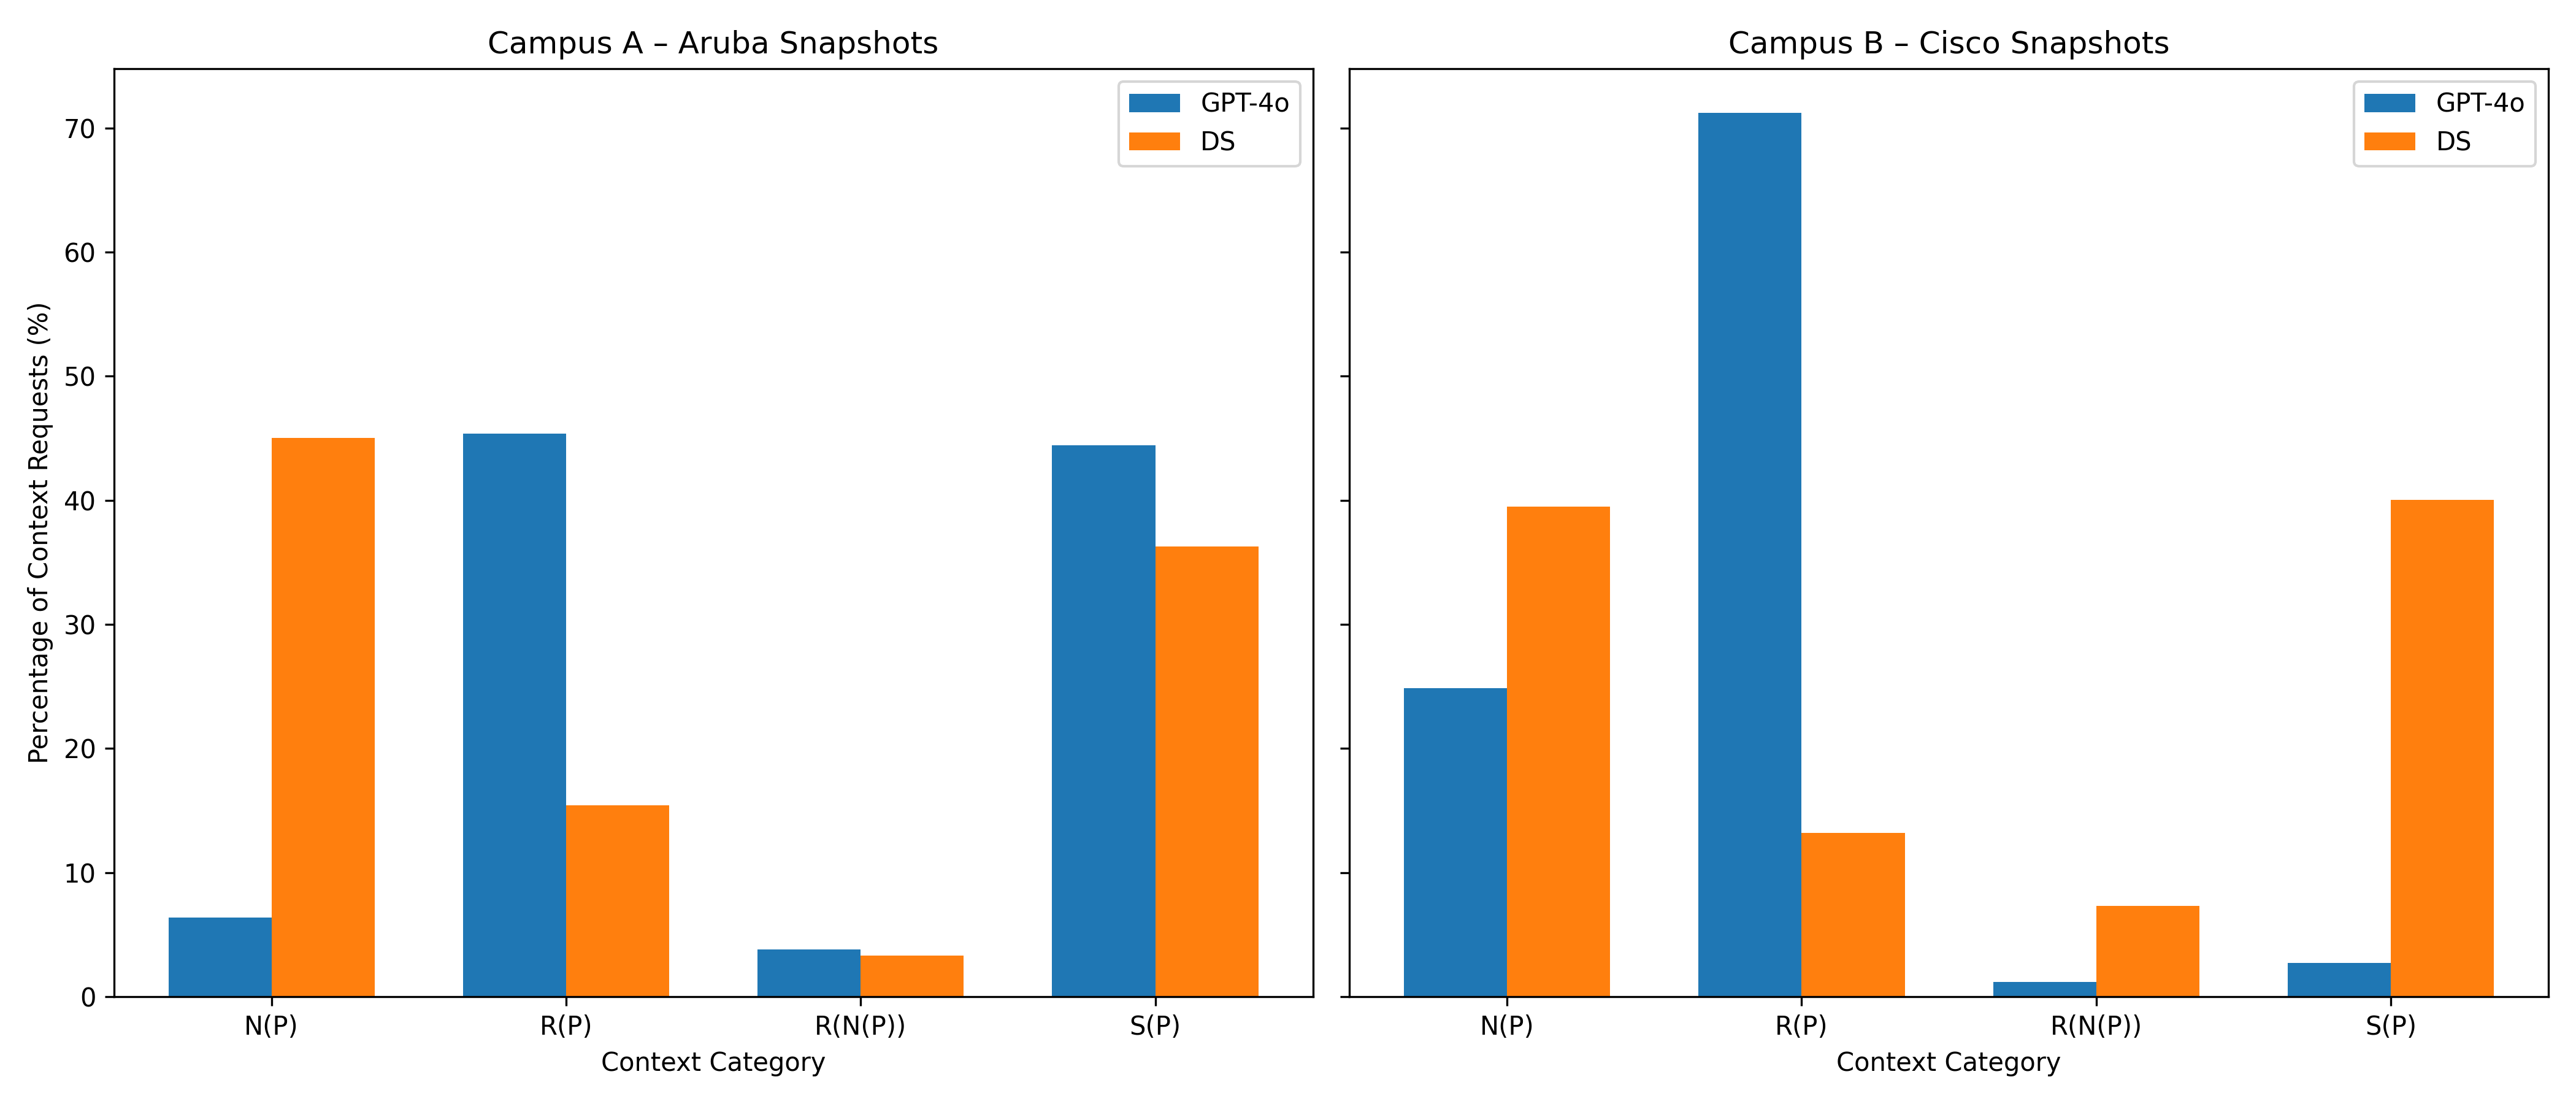
\includegraphics[width=\linewidth]{figs/context_usage_campus_a_b_combined.png}
    \caption{Distribution of context categories requested by GPT-4o and DS, visually highlighting their different analysis strategies.}
    \label{fig:context-usage}
\end{figure*}


\mypara{Implications for Framework Design and Model Choice:}
These observations highlight that the false positives observed in \sysname{} are not artifacts of random noise—they are direct reflections of each model’s interpretive strategy.
This raises an important question about our framework design: in letting the LLM choose its own context to avoid information overload, have we risked the model not requesting \textit{enough} context? To quantify this trade-off, we conducted an ablation study comparing our standard "ask-for-context" approach against a "provide-all-context" method on the challenging Campus B dataset. The results, shown in Table~\ref{tab:ablation_results}, confirm that our design is a justified and effective choice. While providing full context significantly reduced GPT-4o's false positives (from 21 down to 5), it did so at the cost of a threefold increase in prompt size. For DeepSeek, the additional context provided no accuracy benefit, only increasing its computational overhead. This study validates that our iterative approach is a more efficient and effective design.


Ultimately, \sysname{}’s explicit, LLM-driven interface provides a transparent foundation for diagnosing such decisions. For a network operator, the choice of model would depend on their goal: GPT-4o's high-recall approach may be preferable for deep, exploratory audits where finding every potential issue is critical, even at the cost of reviewing false alarms. In contrast, DeepSeek's high-precision approach is better suited for continuous, automated checks where minimizing false positives and operator alerts is the primary concern.

\subsection{How Does \sysname{} Compare to Existing Tools?}

Finally, we compare \sysname{}'s performance against four representative state-of-the-art tools using the synthetic misconfiguration dataset from Internet2. This controlled setting, with its clearly defined ground truth, allows for a direct, feature-by-feature comparison. The tools include:
\begin{itemize}
    \item Two consistency checkers: \textit{Batfish}~\cite{fogel2015general} and \textit{Diffy}~\cite{kakarla2024diffy}.
    \item Two alternative LLM-based approaches: a full-file prompting model (\textit{FFP}) and the partition-based Q\&A model \textit{Ciri}~\cite{lian2023configuration}.
\end{itemize}
For a fair comparison, both FFP and Ciri use the same \textbf{GPT-4o} backend as \sysname{} in this experiment. We do not compare against formal model checkers because no specification of forwarding requirements is available for these networks.

The results in Table~\ref{tab:syn_result} demonstrate that \sysname{} significantly outperforms the other tools in detecting all three types of misconfigurations. It achieves a perfect 16/16 detection rate for erroneous configurations and a 100\% accuracy rate overall. This indicates that \sysname{}'s comprehensive context mining and iterative prompting process effectively identify errors, even in complex D/C cases where other tools struggle.

\begin{table}[t]
\centering
\resizebox{0.8\columnwidth}{!}{
\begin{tabular}{|l|l|c|c|}
\hline
\textbf{Model} & \textbf{Framework Version} & \textbf{False Positives} & \textbf{Avg. Context Tokens} \\
\hline
\multirow{2}{*}{GPT-4o} & \sysname{} (Standard) & 21  & $\sim$ 180 \\
 & \sysname{}-FullContext & 5 & $\sim$ 650 \\
\hline
\multirow{2}{*}{DeepSeek-V3} & \sysname{} (Standard) & 4  & $\sim$ 148 \\
 & \sysname{}-FullContext & 4  & $\sim$ 590 \\
\hline
\end{tabular}
}
\caption{Ablation study results on the Campus B dataset, comparing the standard iterative \sysname{} framework against a version that provides all context by default.}
\label{tab:ablation_results}
\end{table}

\begin{table*}[t]
\centering
\resizebox{\columnwidth}{!}{
\begin{tabular}{|l|l|l|l|l|l|l|}
\hline
\multirow{2}{*}{\textbf{Type}} & \multirow{2}{*}{\textbf{Cases}} & \multicolumn{5}{c|}{\textbf{Number of Detected Misconfigurations}} \\ \cline{3-7} 
&                       & \textbf{\sysname{}} & \textbf{Ciri}& \textbf{FFP} & \textbf{Batfish} & \textbf{Diffy} \\ \hline
Syntax Error & 4 & 4/4 (100\%) & 2/4 (50\%) & 0/4 (0\%) & 3/4 (75\%) & 0/4 (0\%) \\ \hline
Range Error & 4 & 4/4 (100\%) & 2/4 (50\%)& 0/4 (0\%) & 0/4 (0\%) & 0/4 (0\%) \\ \hline
D/C Error& 8 & 8/8 (100\%) & 1/8 (12.5\%) & 0/8 (0\%)& 2/8 (25\%) & 0/8 (0\%) \\ \hline
\multirow{2}{*}{\makecell[{{l}}]{Correct Config\\ Updates}}& \multirow{1}{*}{\makecell[{{l}}]{16}} & \multirow{2}{*}{\makecell[{{l}}]{0/16 (0\%)}} & \multirow{2}{*}{\makecell[{{l}}]{0/16 (0\%)}} & \multirow{2}{*}{\makecell[{{l}}]{13/16 (81.2\%)}}& \multirow{2}{*}{\makecell[{{l}}]{0/16 (0\%)}} & \multirow{2}{*}{\makecell[{{l}}]{0/16 (0\%)}} \\ 
& (False Positives) & & & & & \\ \hline
\textbf{Total Accuracy} & \textbf{32} & \textbf{32/32 (100\%)} & \textbf{21/32 (65.6\%)} & \textbf{19/32 (59.4\%)} & \textbf{21/32 (65.6\%)} & \textbf{16/32 (50\%)} \\ \hline
\end{tabular}}
\caption{Comparison of misconfiguration detection on the synthetic dataset. The "Correct Config Updates" row indicates the number of false positives. Lower is better for that row.}
\label{tab:syn_result}
\end{table*}

\mypara{Comparison Against LLM-based Approaches}
The partition-based GPT model, Ciri, performs reasonably well in detecting syntax and range violations (50\% for both). This success is attributable to the LLM's training on vast amounts of text, including network documentation, which allows it to recognize common, localized structures. However, Ciri lags significantly in detecting D/C issues (12.5\%) because its partitioning approach analyzes configuration sections in isolation, failing to capture the complex interdependencies between distant configuration lines that are crucial for detecting such errors.
Full-File Prompting (FFP) attempts to overcome partitioning by providing the entire configuration in a single query, but it proves even less effective, failing to detect any true misconfigurations. Its primary drawbacks are \textit{token limitations}—where large configurations are truncated—and \textit{context overload}, where excessive information prevents the model from prioritizing relevant details.

By dynamically retrieving only the necessary context based on the LLM's requests (as shown in Table~\ref{tab:syn_configs}), \sysname{} eliminates the fragmentation issues of partition-based methods while avoiding the information saturation problem of FFP. This ensures the model receives a focused yet holistic view of configuration interdependencies, dramatically improving its ability to identify complex misconfigurations.

\mypara{Comparison Against Non-LLM-based Tools}
Batfish performs well on syntax errors (75\% detection rate) but struggles with range violations (0\%) and only partially detects D/C issues (25\%). As a consistency checker, Batfish verifies configurations against a predefined set of best practices and structural rules. This makes it effective at catching explicit errors like missing keywords (which a device CLI might also catch) or references to non-existent groups hard-coded in its rules. However, it is less capable of handling misconfigurations that require deeper contextual reasoning, such as policy conflicts or semantic range violations that are not covered by its rules.

Diffy performs poorly across all misconfiguration types (0\% detection rate). Its data-driven approach focuses on learning common usage patterns and flagging structural anomalies. While our misconfigurations do represent deviations, they are often semantic rather than structural. For instance, an invalid MTU value is numerically incorrect but does not alter the configuration's structure, making it difficult for Diffy’s template-based anomaly detection to capture without a granular understanding of parameter constraints.

Finally, despite varying performance, the majority of the tools—\sysname{}, Batfish, Diffy, and Ciri—successfully marked all 16 correct updates as valid, demonstrating strong capabilities in avoiding false positives. However, FFP failed in this aspect, falsely classifying 13 out of 16 correct updates as misconfigurations. This hallucination likely stems from FFP’s inability to effectively filter relevant information within a large configuration file, leading the model to generate erroneous assessments.

While a direct comparison on the Campus A and B configurations would be valuable, many of the novel issues found by \sysname{} (\eg, ambiguous rate limits, insecure but syntactically valid algorithms) are semantic or policy-related issues that fall outside the designed scope of traditional consistency checkers and pattern-based tools. The synthetic dataset thus provides a fairer and more controlled basis for comparison.